%%%%%%%%%%%%%%%%%%%%%%%%%%%%%%%% Introducción:
\begin{frame}[fragile]{Categorías.}{}
  Existen dos categorías principales para realizar agrupamientos:
  \begin{enumerate}
  \item \textbf{Algoritmos de agrupamiento \textit{jerárquico}}.
    \begin{enumerate}
    \item Aglomerantes.
      
      Inicialmente cada objeto es un grupo, conforme transcurren las
      iteraciones los objetos se deben ir fucionando.
    \item Divisivos.
      
      Inicialmente todos los objetos son un solo grupo, conforma transcurren
      las iteraciones se van subdividiendo estos grupos.
    \end{enumerate}
  \item \textbf{Algoritmos de agrupamiento \textit{particional}}.
    
    Cada objeto se asocia con el centro de agrupamiento del más cercano.
  \end{enumerate}
  \begin{figure}
    \centering
    \begin{subfigure}[b]{0.4\textwidth}
      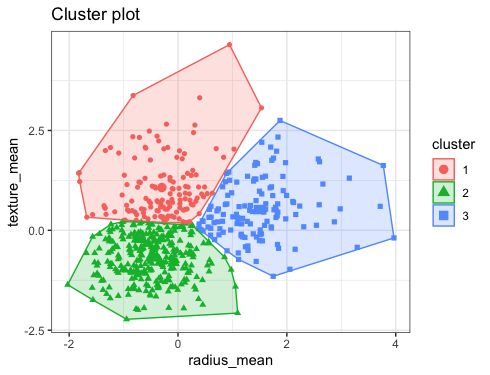
\includegraphics[width=\textwidth]{./Imagenes/kmeans.png}
      \caption*{Agrupamiento Particional.}
    \end{subfigure}
    \begin{subfigure}[b]{0.3\textwidth}
      \includegraphics[width=\textwidth]{./Imagenes/jerarquico.png}
      \caption*{Agrupamiento Jerárquico.}
    \end{subfigure}
  \end{figure}
\end{frame}
